
\documentclass[11pt, a4paper, slovene]{book}

%%%%%% PACKAGES %%%%%%
\usepackage[slovene]{babel}
\usepackage[utf8]{inputenc}
\usepackage{lmodern}
\usepackage[T1]{fontenc}
\usepackage{fancyhdr}
\usepackage{caption}
\captionsetup{font={default,footnotesize}, labelfont=bf, format=hang,indention=.0cm}
\usepackage{graphicx,epsfig}
\usepackage{epstopdf}
\usepackage{amsmath}
\usepackage{multirow}
\usepackage{color}
\usepackage{url}
\usepackage{makeidx}
\usepackage[official]{eurosym}
\usepackage[euler]{textgreek}
\usepackage{listings}
\usepackage[normalem]{ulem}
\usepackage{array}
\usepackage{float}

\begin{document}
\chapter{Modeliranje TCP/IP omrežij}
\chapterauthor{Matevž Ogrinc, Robert Modic, Andreja Kovačič}
\section{Uvod}

TCP/IP je model računalniškega omrežja, ki pove kako morajo biti podatki
zapakirani, naslovljeni, poslani, usmerjeni in prejeti v končnem vozlišču.
Največ omrežnega prometa poteka preko protokola TCP. Preko njega se sporočila zaradi vzpostavljene povezave med odjemalcem in servisom prenašajo zanesljivo v obe smeri, so brez napak, podvojevanja in v pravem vrstnem redu. Ker je TCP povezovalni protokol, se najprej vzpostavi povezava med odjemalcem in strežnikom. Pri povezavi je določen odjemalčev naslov IP in vrata (vrata lahko zavzemajo vrednost od 1 do vključno 65535), ter strežnikov naslov IP in vrata na katerih posluša servis strežnika. Naslov IP povezan z določenimi vrati tvorita vtičnico (socket) in par odjemalčeve in strežnikove vtičnice tvorita povezavo TCP, ki je edinstveno določena. Glava (header) paketa TCP vsebuje izvorni naslov IP in vrata, ciljni naslov IP in vrata, zaporedna številka paketa, številka potrditve in kontrolne zastavice. Kontrolni zastavici, pomembni za gradnjo požarnega zidu sta ACK in SYN. Drug del prometa se prenaša preko protokola UDP, ta ne zagotavlja prenosa podatkov tako kot to zagotavlja TCP, vendar je zato mnogo hitrejši. UDP se zato uporablja kadar ne potrebujemo vseh poslanih paketov, ne dovolimo pa veliko zamude pri njihovem prejemanju. Tako je primeren za prenose raznih multimedijskih vsebin.


\section{Gradniki za realizacijo IPv4 omrežij}
	\begin{itemize}
		\item\textit{IPv4}: glavni modul, ki implementira IP protokol(RFC 791). Modul izvaja enkapsulacijo, dekapsulacijo, fragmentacijo in defragmentacijo in usmerjanje IP datagramov. Prispeli paketi se posredujejo v ARP modul. Privzeta predpostavka modula je, da se vsi paketi obravnavajo enako dolgo, brez prioritet. Za drugačne nastavitve je treba spremeniti implementacijo.
		\item\textit{IPv4RoutingTable}: pomožni modul, ki skrbi za usmerjevalne tabele vozlišč. Vsak gostitelj in usmerjevalki vsebuje eno kopijo. Modulu IPv4 dostavlja podatke o najboljših poteh, posodabljajo pa ga daemoni RIP, OSPF, Manet in drugih protokolov. Modul nima vrat, vsa komunikacija z njim poteka skozi klice funkcije (predvsem read in update). Ko je na voljo več poti za dan naslov, se upošteva pot:
		z najdaljšim ujemanjem naslova,z najbolj specifično multicast skupino, z najmanjšo metriko (ceno poti).
		\item\textit{ICMP}: modul generira ICMP(RFC 792) pakete, podpira echo aplikacije. ICMP protokol se uporablja za spetno javljnje napak in diagnostiko. Ker uporablja protokol IP, spada med transportne protokole, vendar se za razliko od TCP/UDP protokolov ne uporablja za prenos uporabnikovih podatkov.
		\item\textit{ARP}: izvaja dinamično prevajanje med lokalnimi naslovi(tipično IP) in strojnimi naslovi(MAC), implementira RFC 826. Inet-ova implementacija podpira samo preslikavo IP-MAC.
		\item\textit{IGMPv2}: Modul generira in procesira multicast sporočila o članstvu odjemalcev v multicast skupine. Podatke posreduje usmerjevalnikom v omrežju. Ko se vmesnik gostitelja želi včlaniti v skupino, pošlje IGMP poročilo vmesniku multicast usmerjevalnika, ta ga obdela in posodobi tabelo naslovnikov multicast sporočil. Podoben postopek je ob izstopu gostitelja iz skupine.
	\end{itemize}

Moduli so sestavljeni v \textit{IPv4NetworkLayer}, ki predstavlja celotno omrežno plast. Ima vrata za TCP, UDP, SCTP, RSVP in druge protokole.  Nanj se lahko povežejo omrežni vmesniki: Ethernet, PPP, Wlan ali drugi zunanji vmesniki. Modul se uporablja za gradnjo gostiteljev(hosts) in usmerjevalnikov (routers).


\section{Zgledi IPv4 omrežij v OMNeT++}
\subsection{Primer 1 - Multicast}

\large \bf Opis omrežja in gradnikov
\normalfont \normalsize 

Multicast omrežje je sestavljeno iz štirih usmerjevalnikov (tipa Router) in šestih odjemalcev (tipa StandardHost). Prikazuje pretok paketov, ki so namenjeni enemu naslovniku torej unicast hkrati pa tudi večim naslovnikom, ki spadajo v skupine ali multicast skupine. Paketi so duplicirani v usmerjevalniku samo v primeru kadar obstajajo poslušalci v njegovem omrežju. Torej usmerjevalnik vnaprej pozna poslušalce določenih multicast skupin. To dosežemo z uporabo protokol v našem primeru IGMPv2, saj IPv4 takega delovanja ne podpira sam po sebi.
\begin{figure}[h]
	\centering
	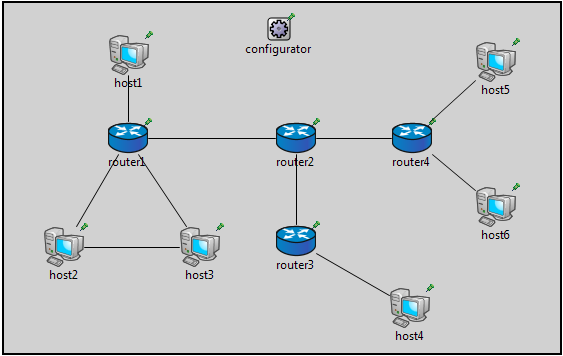
\includegraphics[width=\textwidth]{Multicast.png}
	\caption{Omrežje Multicast in njegovi gradniki}
	\label{Multicast}	
\end{figure}
\pagebreak

\large\bf Podrobna analiza
\normalfont \normalsize 

Ob zagonu simulacije opazimo pakete tipa IGMPv2Query iz tako imenovanega glavnega usmerjevalnika v našem primer je to usmerjevalnik2 (router2), ki predstavlja povpraševanje po obstoječih poslušalcev multicast naslovov, nato kot odgovor iz vsakega od vozlišč opazimo paket IGMPv2Report. Ob prejemu tega paketa lahko glavni usmerjevalnik ustvari multicast tabelo, saj mu pove ali obstaja poslušalec za nek multicast naslov. Tabela usmerjevalniku pove, ob prispelem multicast paketu, ali naj paket pošlje naprej ali ne in kam. Ob končani poizvedbi se prične normalni pretok multicast paketov do odjemalcev oz poslušalcev. Če pogledamo glavni usmerjevalnik opazimo, da vsebuje njegova multicast tabela tri multicast skupine: 
\begin{enumerate}
	\item (127.0.0.x) s poslušalci host1,host2 in host3 ter usmerjevalnikom 1
	\item (127.0.1.x) s poslušalcem host4 in usmerjevalnikom 3
	\item (127.0.2.x) za poslušalca host5, host6 in usmerjavalnikom 4
\end{enumerate} 
\subsection{Primer 2 - Flatnet}
\large \bf Opis omrežja in gradnikov
\normalfont \normalsize 

Omrežje je sestavljeno iz enega strežnika, 57 usmerjevalnikov in dveh odjemalcev. Namen tega omrežja je prikazati avtomatsko sestavo routing tabele in dodeljevanje IP naslovov, hkrati pa tudi prikaže proces three-way handshake-a med odjemalcem in strežnikom za prenos podatkov. Omrežje ima dve vrsti povezovanja, preko Ethernet kabla in optike. Zaradi velike količine usmerjevalnikov bomo omrežje ponazorili z spodnjo sliko.
\begin{figure}[h]
	\centering
	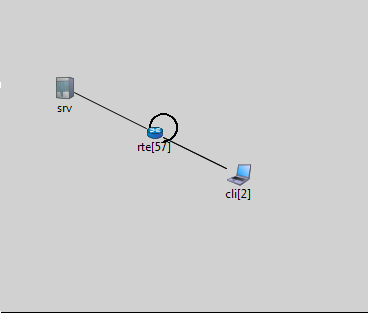
\includegraphics{FlatNet.png}
	\caption{Omrežje FlatNet in njegovi gradniki}
	\label{flatNet}	
\end{figure}
\pagebreak
\large\bf Analiza flatnet
\normalfont \normalsize 

Ob zagonu simulacije se pošljejo iz odjemalca SYN paketi oz Synchronization packets. Paketi potujejo po usmerjevalni tabeli od usmerjevalnikov do strežnika kjer nato strežnik odgovori z SYN-ACK oz acknowledge paketi, ki potujejo po istih usmerjevalnikih nazaj. Ob prejemu SYN-ACK paketa odjemalec odgovori z istim SYN-ACK paketom. SYN paketi se uporabljajo za vzpostavitev three-way handshake procesa v TCP-ju. To se zgodi kadar odjemalec želi pošiljati drugemu odjemalcu podatke. Po three-way handshake procesu odjemalec začne pošiljati podatke v obliki TCP segmentov. Ob prejemu teh se strežnik odzove z ACK oz acknowledge paketi. Celoten proces se zgodi za oba odjemalca. S to razliko da eden uporablja ethernet, drugi pa optično povezavo. Omrežje deluje zato, ker ima avtomatsko dodeljevanje IPv4 naslovov in avtomatsko kreirane usmerjevalne tabele, da lahko paketi pridejo do cilja.


\subsection{Primer 3 - Bulktransfer}
\large \bf Opis omrežja in gradnikov
\normalfont \normalsize 

Omrežje je sestavljeno iz enega usmerjevalnika, tremi odjemalci in enim strežnikom. Namen je prikazati uporabo TCP client/Server modele za prenos večjih datotek ali "Bulktransfer". Dva odjemalca sta povezana z strežnikom preko usmerjevalnika, eden je pa povezan direktno, kot je razvidno na spodnji sliki.
\pagebreak
\begin{figure}[h]
	\centering
	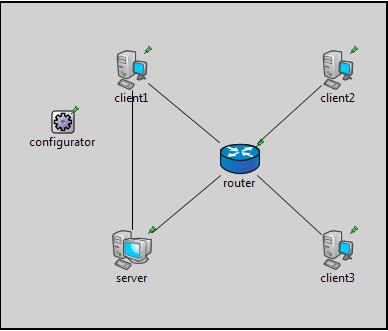
\includegraphics[width=\textwidth]{BulkTransfer.png}
	\caption{Omrežje bulktransfer in njegovi gradniki}
	\label{bulkTransfer}	
\end{figure}

\large\bf Analiza bulktransfer
\normalfont \normalsize

Ob zagonu simulacije se iz odjemalca(client 1) pošlje Syn paket za three-way handshake s strežnikom. Ob istem času pa iz odjemalca (client 2 in client 3) prihaja isti SYN paket najprej za usmerjevalnik nato usmerjevalnik SYN paket pošlje do strežnika. Vsi trije odjemalci prejmejo SYN-ACK pakete in opravijo three-way handshake z strežnikom. Nato odjemalci pošljejo na strežnik maksimalno velike pakete ter jih hkrati od strežnika tudi prejemajo. Ob prejemu TCP segmenta pošljejo strežniku ali strežnik njim ACK. potrditev, da so segment prejeli. Za prenos moramo večje datoteke razdeliti na segmente in jih po delih pošiljati do strežnika, kar ta simulacija tudi ponazarja.



\section{Načrtovanje omrežij}
\subsection{Omrežje 1,2}
\large \bf Opis 
\normalfont \normalsize

Omrežje je sestavljeno iz enega serverja in 5*n odjemalcev, n se prilagaja za simulacijo obremenitve omrežja. Vsi odjemalci pošiljajo ping sporočila na server, izvajajo naiven denial of service napad. Prva verzija omrežja nima optične hrbtenice, druga jo ima med usmerjevalniki 2,5,6. 
Namen simulacije je ugotoviti, kako hrbtenica pripomore k posredovanju paketov do končnega naslovnika.

\begin{figure}[h]
	\centering
	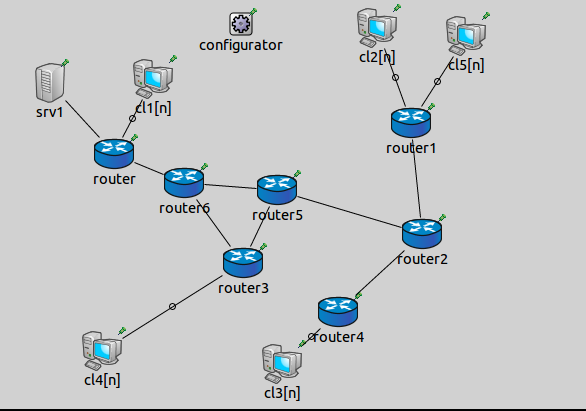
\includegraphics[width=\textwidth]{omrHrbet.png}
	\caption{Omrežje z optično hrbtenico}
	\label{opticnaHrbtenica}	
\end{figure}

\subsection{Omrežje 3}
\large \bf Opis 
\normalfont \normalsize

Omrežje je sestavljeno iz enega serverja (standardHost), šestih usmerjevalnikov (router-router6) in vsak usmerjevalnik ima določeno število odjemalcev. Usmerjevalnik 6 (router6) ima z razliko od ostalih usmerjevalnikov 5 odjemalcev (razen usmerjevalnik, ki povezuje ostale usmerjevalnike z strežnikom). Povezave v omrežju so bakrene (z hitrostjo 10Mbps)

\begin{figure}[h]
	\centering
	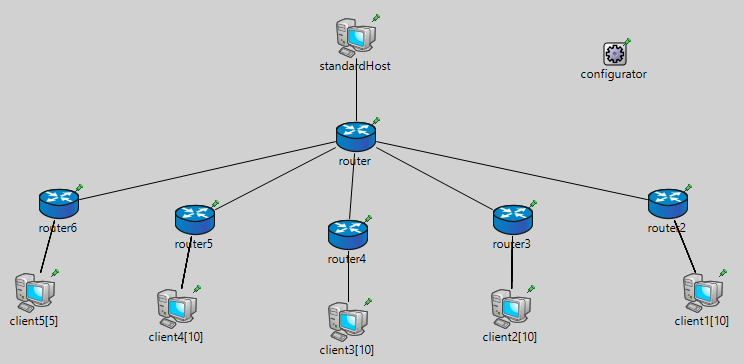
\includegraphics[width=\textwidth]{server_client.png}
	\caption{Omrežje 2 z TCP protokolom}
	\label{omrezje2}	
\end{figure}
\pagebreak
\subsection{Omrežje 4}
\large \bf Opis 
\normalfont \normalsize

Kot vidimo iz spodnje slike je podano omrežje enako Omrežju 2 z razliko, da uporablja udp Protokol. Omrežje je sestavljeno iz enega serverja (standardHost), šestih usmerjevalnikov (router-router6) in vsak usmerjevalnik ima določeno število odjemalcev. Usmerjevalnik 6 (router6) ima z razliko od ostalih usmerjevalnikov 5 odjemalcev (razen usmerjevalnik, ki povezuje ostale usmerjevalnike z strežnikom). Povezave v omrežju so bakrene (z hitrostjo 10Mbps).

\begin{figure}[h]
	\centering
	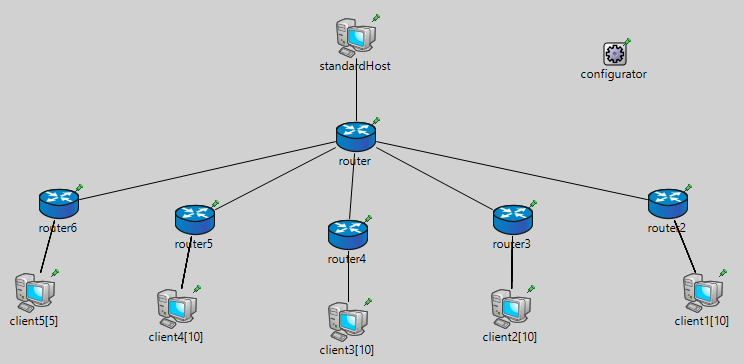
\includegraphics[width=\textwidth]{server_client.png}
	\caption{Omrežje 3 z UDP protokolom}
	\label{omrezje3}	
\end{figure}


\section{Analiza Omrežij} 
\subsection{Simulacija} 
\large \bf Opis simulacij 
\normalfont \normalsize

Omrežja smo simulirali z tremi vrstami teoretičnih obremenitev: nadpovprečni obremeniti, povprečni obremenitvi in podpovprečni obremenitvi. Za simuliranje vseh tipov obremenitev bomo povečali/zmanjšali število in pa hitrost pošiljanja paketov od odjemalcev. Simulacije so trajale 120s.  

\subsection{Izbira statistik} 
\large \bf Opis statističnih parametrov 
\normalfont \normalsize

Za vse simulacije smo se odločili opazovati specifične statistične metrike, ki nam bodo povedali kakovost in delovanje omrežja. To so

\begin{enumerate}
	\item Povprečni čas čakanja paketov v čakalni vrsti
	\item Število izgubljenih paketov na določenih usmerjevalnikih
	\item RTT
\end{enumerate}

Hkrati pa smo spreminjali naslednje parametre na simulacijah, saj smo s spremembami bolje videli razliko v delovanju omrežja

\begin{enumerate}
	\item Dolžina čakalnih vrst
	\item Frekvenco pošiljanja paketov
	\item Hitrost strežbe paketov
\end{enumerate}


	
\subsection{Rezultati in analiza simulacij}

\subsection{Ping omrežje brez hrbtenice}

Podpovprečno obremenitev smo simulirali s 75 odjemalci, omrežje ni imelo hrbtenice, tako so bile vse povezave enako močne - 10Mb/s. Čakalne vrste so lahko sprejele največ dva paketa. Iz spodnjega grafa je razvidno, da kljub krajši čakalni vrsti ni prihajalo do izgube paketov. S spremebo dolžin čakalne vrste na 10 paketov tako nismo dosegli nikakršnega učinka, nasprotno pa je podaljšanje obdelave paketa zvišalo tako RTT kot čas v čakalnih vrstah. 

\begin{figure}[h]
	\centering
	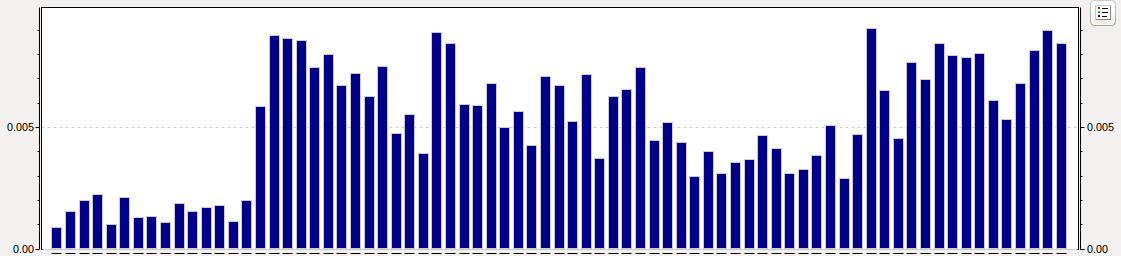
\includegraphics[width=\textwidth]{lRtt1.png}
	\caption{RTT paketov v podpovprečno obremenjenem omrežju, na x osi so klienti, na y osi RTT v sekundah.}
	\label{RTT1}	
\end{figure}
\pagebreak
Povprečno obremenitev smo simulirali z 175 odjemalci, sicer so simulacije potekale z enakimi parametri kot podpovprečno obremenjeno omrežje. Tudi v tem primeru čakalne vrste z največ dvema paketoma niso povzročile izgube paketov, je pa dvakrat višji RTT. Deset mest v čakalni vrsti tako spet ni povzročilo razlike, polovično višanje časa obdelave paketov pa je povzročilo manjše izgube paketov.

\begin{figure}[h]
	\centering
	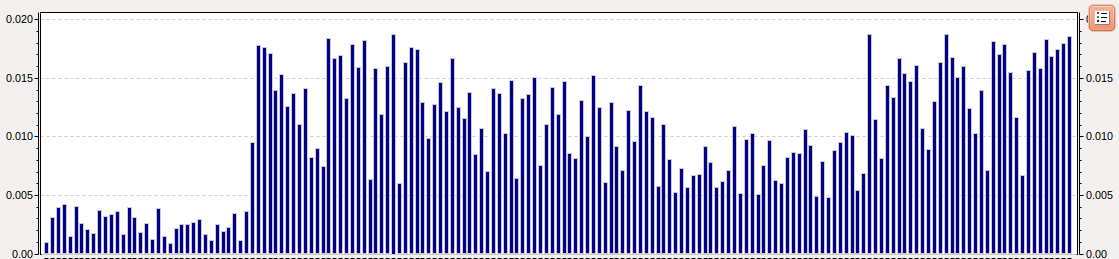
\includegraphics[width=\textwidth]{aRtt1.png}
	\caption{RTT paketov v povprečno obremenjenem omrežju. Na x osi klienti, na y RTT v sekundah.}
	\label{RTT2}	
\end{figure}

Nadpovprečna obremenitev je zajemala 750 odjemalcev. Prišlo je do velike izgube paketov, zato povprečni RTT v tem primeru ne pove veliko.  V primeru 10 mest v čakalnih vrstah do izgub ne prihaja, RTT pa se linearno povečuje. Spodaj je prikazan RTT v omrežju z 2 mestoma 

\begin{figure}[h]
	\centering
	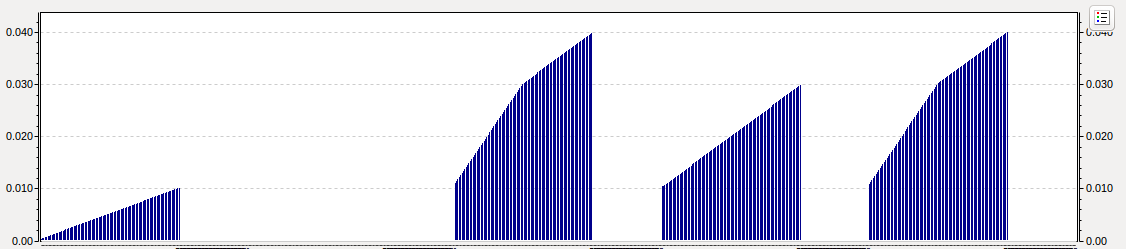
\includegraphics[width=\textwidth]{hRtt1.png}
	\caption{RTT paketov v nadpovprečno obremenjenem omrežju, na x osi so klienti, y prikazuje povprečen RTT v sekundah.}
	\label{RTT3}	
\end{figure}

\begin{figure}[h]
	\centering
	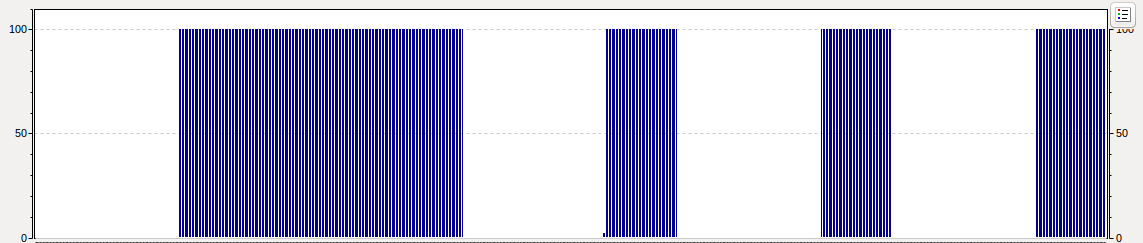
\includegraphics[width=\textwidth]{hPL1.png}
	\caption{Delež izgubljenih paketov v nadpovprečno obremenjenem omrežju, x os prikazuje kliente, y delež izgubljenih paketov.}
	\label{hPL1}	
\end{figure}
\pagebreak

\subsection{Ping omrežje s hrbtenico} 

Hrbtenico smo simulirali na dveh povezavah, med usmerjevalniki 2,5 in 6, hitrost povezav je bila 512 Mbps, sicer 10 Mbps. 

Za podpovprečno obremenitev smo uporabili 75 klientov, izgub paketov ni bilo ne glede na dolžino čakalnih vrst, tudi ob polovičnem zmanjšanju hitosti obdelave paketov ne. 

\begin{figure}[h]
	\centering
	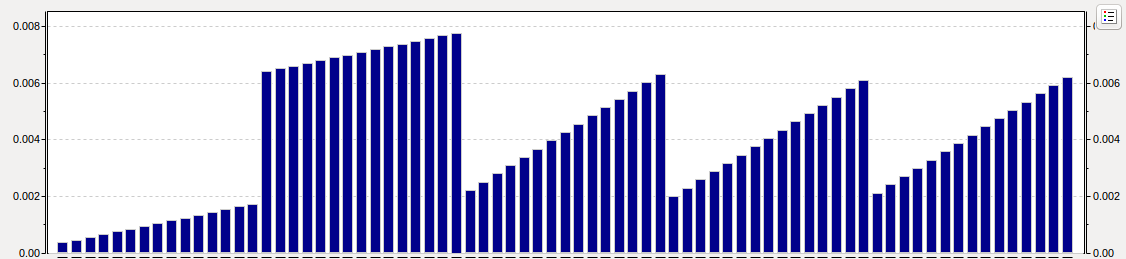
\includegraphics[width=\textwidth]{lRtt2.png}
	\caption{RTT paketov v podpovprečno obremenjenem omrežju s hrbtenico. Na x osi klienti, na y RTT v sekundah.}
	\label{RTT4}	
\end{figure}

Povprečna obremenitev s 150 klienti ni utrpela izgub, ne glede na dolžino čakalnih vrst ali spremebe dolžine obdelave paketov.
\begin{figure}[h]
	\centering
	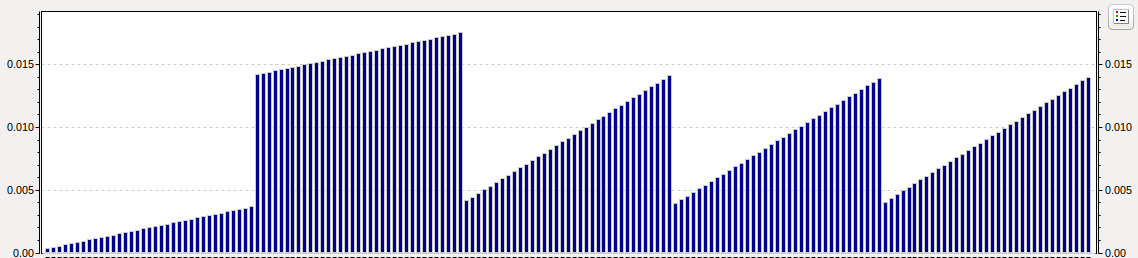
\includegraphics[width=\textwidth]{aRtt2.png}
	\caption{RTT paketov v povprečno obremenjenem omrežju s hrbtenico. Na x osi klienti, na y osi RTT v sekundah.}
	\label{RTT5}	
\end{figure}

\pagebreak

Nadpovprečna obremenitev s 750 klienti tudi ob pomoči hrbtenice izgublja precej paketov, ob podaljšanju čakalnih vrst na 10 mest je izguba paketov praktično ničelna X.

\begin{figure}[h]
	\centering
	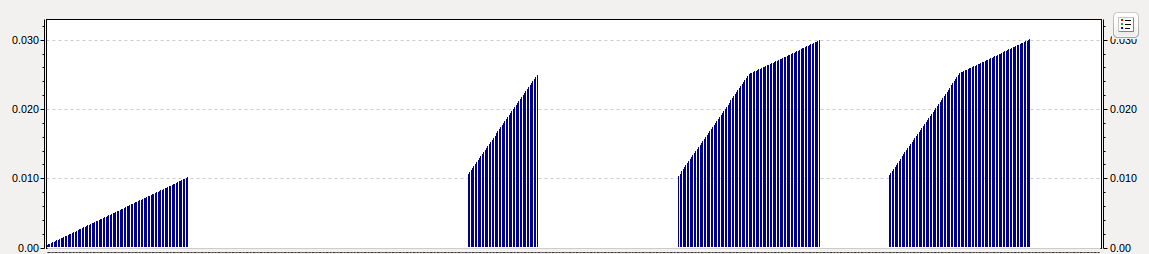
\includegraphics[width=\textwidth]{hRtt2.png}
	\caption{RTT paketov v nadpovprečno obremenjenem omrežju s hrbtenico. Na x osi so klienti, na y RTT v sekundah.}
	\label{RTT6}	
\end{figure}

\begin{figure}[h]
	\centering
	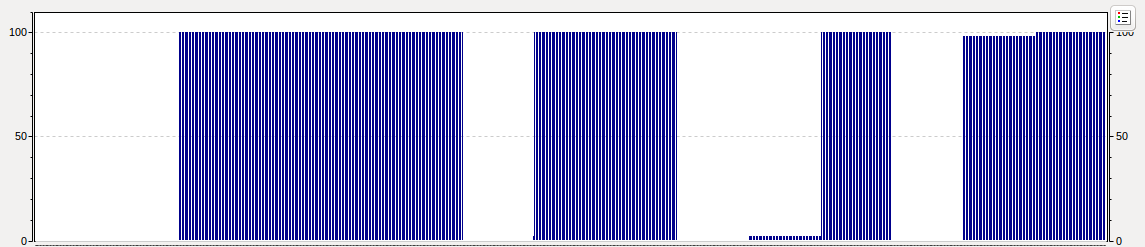
\includegraphics[width=\textwidth]{hLoss2.png}
	\caption{Delež izgubljenih paketov v nadpovprečno obremenjenem omrežju s hrbtenico. Na x osi so klienti, y os predstavlja delež.}
	\label{hPL2}	
\end{figure}

\subsection{Primerjava omrežja z optično hrbtenico in brez} 
Optična hrbtenica v vseh simulacijah občutno zmanjša RTT, tudi dvakratno. Do izgub še vedno prihaja, če usmerjevalniki ne zmorejo procesirati vseh paketov - kar prikazujejo grafi nadpovprečno obremenjenih omrežij, kjer izgube dosegajo do 1000 paketov, nekateri klienti niso prejeli odgovora na nobenega od poslanih 50 ping sporočil. Spreminjanje dolžine vrste ni doseglo večjega učnika, sprememba iz 2 na 200 ne reši mnogo več sporočil, ravno zaradi hitrosti pošiljanja klientov.

\begin{figure}[h]
	\centering
	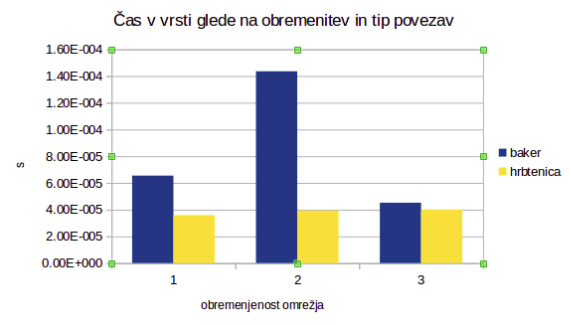
\includegraphics[width=\textwidth]{casObremenitevTip.png}
	\caption{Povprečen čas čakanja v vrsti glede na obremenitev in tip povezav.}
	\label{cOT}	
\end{figure}

\begin{figure}[H]
	\centering
	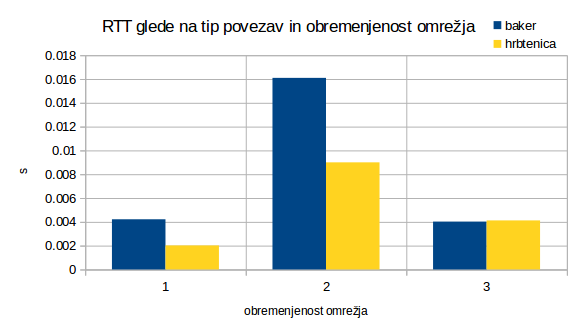
\includegraphics[width=\textwidth]{rttPovezaveObr.png}
	\caption{Povprečen RTT glede na obremenitev in tip povezav.}
	\label{rOT}	
\end{figure}


\subsection{Simulacije omrežja 3 in 4}

\begin{tabular}{|p{3cm}||p{3cm}|p{3cm}|}
	\hline
	\multicolumn{3}{|c|}{Konfiguracija simulacij} \\
	\hline
	Simulacije& Frekvenca/interval pošiljanja paketov& Dolžina čakalne vrste \\
	\hline 
	simulacija 1 (TCP)& 1mb & 100\\
	\hline 
	simulacija 2 (TCP)& 10mb & 100\\
	\hline 
	simulacija 3 (TCP)& 100mb & 100\\
	\hline 	
	simulacija 4 (UDP)& 15ms & 10\\
	\hline 
	simulacija 5 (UDP)& 10ms & 10\\
	\hline 
	simulacija 6 (UDP)& 5ms & 10\\
	\hline 
	simulacija 7 (TCP)& 10mb &	10\\
	\hline 
	simulacija 8 (TCP)& 10mb & 50\\
	\hline
	simulacija 9 (TCP)& 10mb & 100\\
	\hline
	simulacija 10 (UDP)& 10ms & 10\\
	\hline
	simulacija 11 (UDP)& 10ms & 50\\
	\hline
	simulacija 12 (UDP)& 10ms & 100\\
	\hline
\end{tabular} 

\large \bf Podpovprečna obremenitev 
\normalfont \normalsize
Za simulacijo podpovprečne obremenitve smo zmanjšali frekvenco pošiljanja paketov. To se vidi v tabeli pod
simulacijo 1 (TCP) in simulacija 4 (UDP). 

\large \bf Povprečna obremenitev 
\normalfont \normalsize
Za simulacijo povprečne obremenitve smo ravno tako nastavili frekvenco pošiljanja paketov, kar se vidi v tabeli pod simulacijo 2(TCP) in simulacijo 5 (UDP). 

\large \bf Nadpovprečna obremenitev 
\normalfont \normalsize
Za simulacijo nadpovprečne obremenitve smo zmanjšali pasovno širino in povečali frekvenco pošiljanja in ustvarjanja paketov, kar se ravno tako kot v prešnjih dveh primerih vidi v tabeli z simulacijo 3 (TCP) in simulacijo 6 (UDP).

\subsection{Ugotovitve in analiza omrežji 3 in 4}
Glede na prejete podatke iz simulacij, smo prišli do ugotovitve, da vsa omrežja pravilno simulirajo TCP/IP protokol glede na tri teoretične obremenitve (podpovprečna, povprečna in nadpovprečna obremenitev). 
Ob nadpovprečni obremenitvi smo ugotovili, da oba omrežja dosežeta nasičenost. Najbolje se to opazi pri simulaciji udp protokola, ki smo ga zajeli pri grafih \ref{4} in \ref{5} oba grafa prikazujeta obnašanje UDP paketov v treh teoretičnih obremenitvah graf \ref{4} prikazuje povprečni čakalni čas v vrsti in graf \ref{5} število izgubljenih paketov. Nato smo analizirali RTT TCP paketov on povprečni obremenitvi, z različnimi dolžinami čakalne vrste \ref{2} ter ob različnih obremenitvah \ref{3}. Opazili smo, da obremenitve ne vplivajo veliko na RTT tcp paketov, ko pa pride do dolžine čakalne vrste pa se grafi že razlikujejo. Večja kot je čakalna vrsta dlje časa preživijo paketi v omrežju kar je razvidno v grafu \ref{2}. Iz grafa \ref{6} opazimo, da se problem izgube paketov reši z spremembo dolžino čakalne vrste, hkrati pa tudi opazimo, da je optimalna velikost vrste v našem primeru 50, saj se v primeru povprečne čakalne vrste razvidi, da skoraj ni razlike v izgubi paketov kadar imamo večjo velikost vrste. 

\subsection{grafi za omrežji 3 in 4}

\begin{figure}[h]
	\centering
	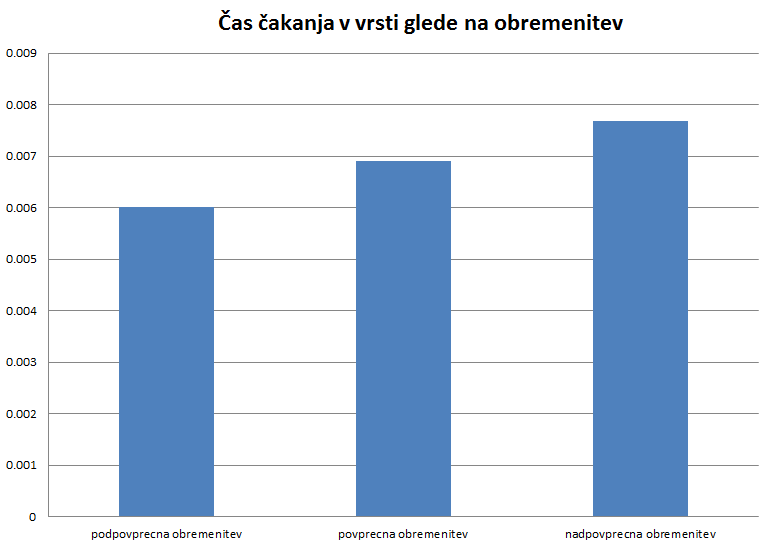
\includegraphics[width=\textwidth]{TCP_cas_vrsta_obremenitev.png}
	\caption{TCP povprečni čas v vrsti glede na obremenitev}
	\label{1}	
\end{figure}


\begin{figure}[h]
	\centering
	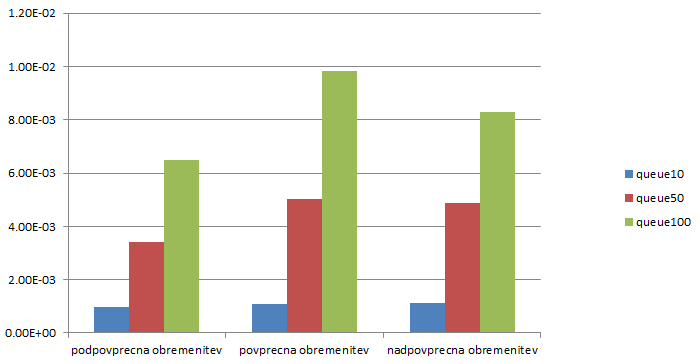
\includegraphics[width=\textwidth]{TCP_RTT_VRSTA_OBREMENITEV.png}
	\caption{TCP RTT-ji glede na dolžino vrste in obremenitve}
	\label{2}	
\end{figure}

\begin{figure}[h]
	\centering
	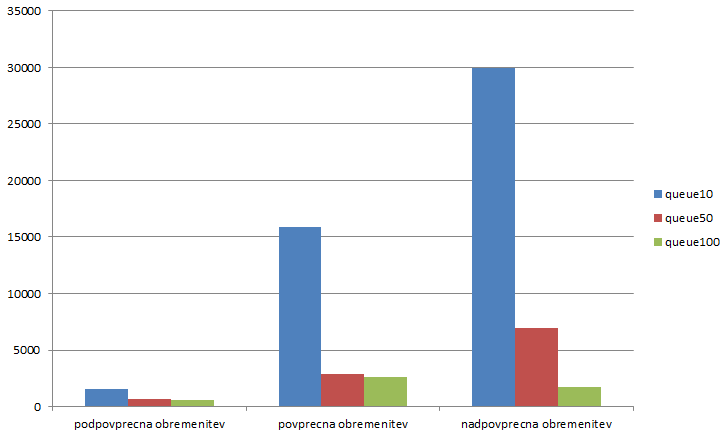
\includegraphics[width=\textwidth]{IZGUBE_PAKETOV_VRSTA_OBREMENITEV.png}
	\caption{TCP izgube paketov glede na dolžino vrste in obremenitve}
	\label{6}	
\end{figure}

\begin{figure}[h]
	\centering
	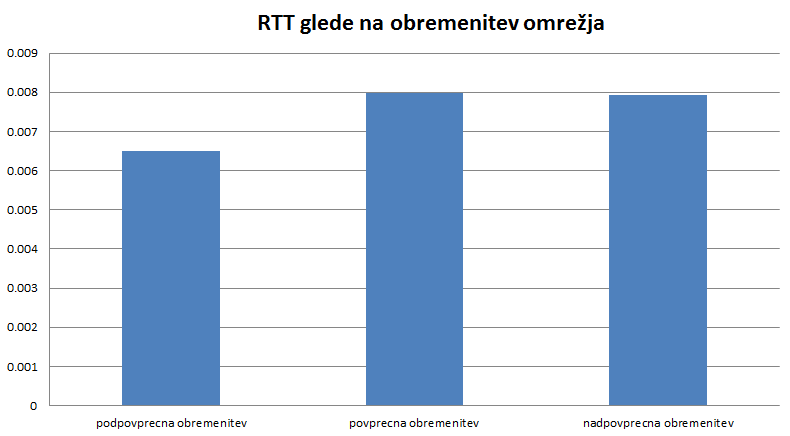
\includegraphics[width=\textwidth]{TCP_RTT_obremenitev_omrezja.png}
	\caption{TCP RTT-ji glede na obremenitev}
	\label{3}	
\end{figure}

\begin{figure}[h]
	\centering
	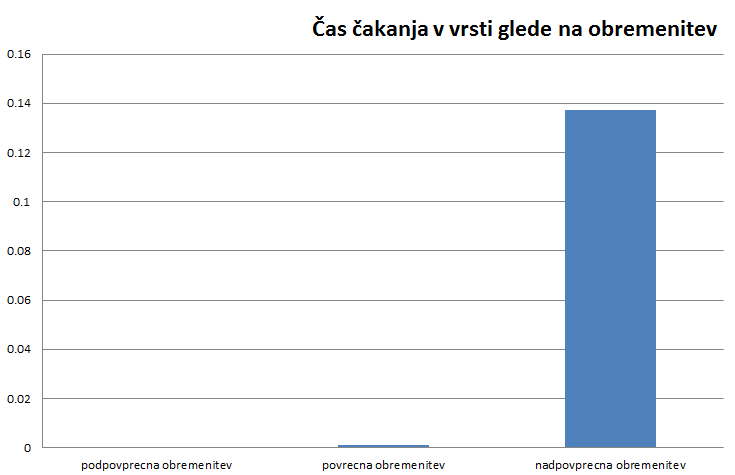
\includegraphics[width=\textwidth]{UDP_cas_cakanja_obremenitev.png}
	\caption{UDP povprečni čas čakanja v vrsti glede na obremenitve}
	\label{4}	
\end{figure}

\begin{figure}[h]
	\centering
	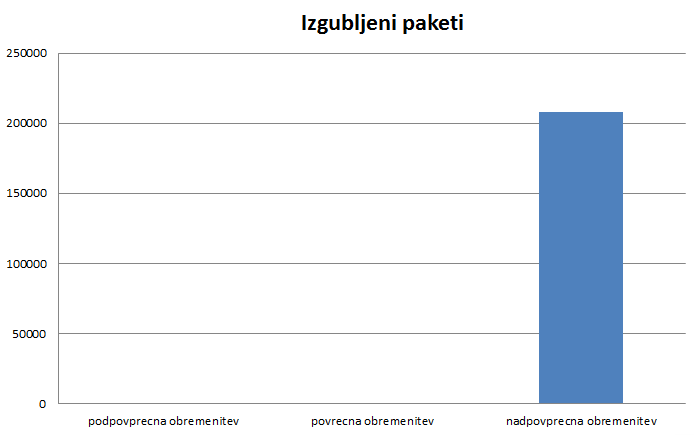
\includegraphics[width=\textwidth]{UDP_izgubljeni_paketi_obremenitev.png}
	\caption{UDP število izgubljenih paketov glede na obremenitev}
	\label{5}	
\end{figure}

\end{document}